%%%%%%%%%%%%%%%%%%%%%%%%%%%%%%%%%%%%%%%%%%%%%%%%%%%%%%%%%%%%%%%%%%%%%%%%
%    INSTITUTE OF PHYSICS PUBLISHING                                   %
%                                                                      %
%   `Preparing an article for publication in an Institute of Physics   %
%    Publishing journal using LaTeX'                                   %
%                                                                      %
%    LaTeX source code `ioplau2e.tex' used to generate `author         %
%    guidelines', the documentation explaining and demonstrating use   %
%    of the Institute of Physics Publishing LaTeX preprint files       %
%    `iopart.cls, iopart12.clo and iopart10.clo'.                      %
%                                                                      %
%    `ioplau2e.tex' itself uses LaTeX with `iopart.cls'                %
%                                                                      %
%%%%%%%%%%%%%%%%%%%%%%%%%%%%%%%%%%
%
%
% First we have a character check
%
% ! exclamation mark    " double quote  
% # hash                ` opening quote (grave)
% & ampersand           ' closing quote (acute)
% $ dollar              % percent       
% ( open parenthesis    ) close paren.  
% - hyphen              = equals sign
% | vertical bar        ~ tilde         
% @ at sign             _ underscore
% { open curly brace    } close curly   
% [ open square         ] close square bracket
% + plus sign           ; semi-colon    
% * asterisk            : colon
% < open angle bracket  > close angle   
% , comma               . full stop
% ? question mark       / forward slash 
% \ backslash           ^ circumflex
%
% ABCDEFGHIJKLMNOPQRSTUVWXYZ 
% abcdefghijklmnopqrstuvwxyz 
% 1234567890
%
%%%%%%%%%%%%%%%%%%%%%%%%%%%%%%%%%%%%%%%%%%%%%%%%%%%%%%%%%%%%%%%%%%%
%
\documentclass[12pt]{iopart}
\newcommand{\gguide}{{\it Preparing graphics for IOP Publishing journals}}
%Uncomment next line if AMS fonts required
%\usepackage{iopams}  
\begin{document}

\title[Author guidelines for IOP Publishing journals in  \LaTeXe]{How to prepare and submit an article for 
publication in an IOP Publishing journal using \LaTeXe}

\author{Content \& Services Team}

\address{IOP Publishing, Temple Circus, Temple Way, Bristol BS1 6HG, UK}
\ead{submissions@iop.org}
\vspace{10pt}
\begin{indented}
\item[]August 2017
\end{indented}

\begin{abstract}
This document describes the  preparation of an article using \LaTeXe\ and 
\verb"iopart.cls" (the IOP Publishing \LaTeXe\ preprint class file).
This class file is designed to help 
authors produce preprints in a form suitable for submission to any of the
journals listed in table~\ref{jlab1} on the next page.  You are not obliged to use this class file---we accept
submissions using all common \LaTeX\ class and style files.  The \verb"iopart.cls"
class file is supplied merely as a convenience for those authors who find it useful.
This document gives both general advice that applies whatever class file you use, and specific advice
that applies if you choose to use \verb"iopart.cls".

We also accept submissions in Word format.  See elsewhere on this site for guidelines on Word submissions.

If you have any queries about this document or any aspect of preparing your article for submission please contact us at the e-mail address given above.
\end{abstract}

%
% Uncomment for keywords
%\vspace{2pc}
%\noindent{\it Keywords}: XXXXXX, YYYYYYYY, ZZZZZZZZZ
%
% Uncomment for Submitted to journal title message
%\submitto{\JPA}
%
% Uncomment if a separate title page is required
%\maketitle
% 
% For two-column output uncomment the next line and choose [10pt] rather than [12pt] in the \documentclass declaration
%\ioptwocol
%



\section{Introduction: file preparation and submission}


The \verb"iopart" \LaTeXe\ article class file is provided to help authors prepare articles for submission to IOP Publishing journals.
  This document gives advice on preparing your submission, and specific instructions on how to use \verb"iopart.cls" to follow this advice.  You
  do not have to use \verb"iopart.cls"; articles prepared using any other common class and style files can also be submitted.
    It is not necessary to mimic the appearance of a published article.

The advice
on \LaTeX\ file preparation in this document applies to
the journals listed in table~\ref{jlab1}.  If your journal is not listed please go to the journal website via \verb"http://iopscience.iop.org/journals" for specific
submission instructions.

\begin{table}
\caption{\label{jlab1}Journals to which this document applies, and macros for the abbreviated journal names in {\tt iopart.cls}. Macros for other journal titles are listed in appendix\,A.}
\footnotesize
\begin{tabular}{@{}llll}
\br
Short form of journal title&Macro name&Short form of journal title&Macro name\\
\mr
2D Mater.&\verb"\TDM"&Mater. Res. Express&\verb"\MRE"\\
Biofabrication&\verb"\BF"&Meas. Sci. Technol.$^c$&\verb"\MST"\\
Bioinspir. Biomim.&\verb"\BB"&Methods Appl. Fluoresc.&\verb"\MAF"\\
Biomed. Mater.&\verb"\BMM"&Modelling Simul. Mater. Sci. Eng.&\verb"\MSMSE"\\
Class. Quantum Grav.&\verb"\CQG"&Nucl. Fusion&\verb"\NF"\\
Comput. Sci. Disc.&\verb"\CSD"&New J. Phys.&\verb"\NJP"\\
Environ. Res. Lett.&\verb"\ERL"&Nonlinearity$^{a,b}$&\verb"\NL"\\
Eur. J. Phys.&\verb"\EJP"&Nanotechnology&\verb"\NT"\\
Inverse Problems&\verb"\IP"&Phys. Biol.$^c$&\verb"\PB"\\
J. Breath Res.&\verb"\JBR"&Phys. Educ.$^a$&\verb"\PED"\\
J. Geophys. Eng.$^d$&\verb"\JGE"&Physiol. Meas.$^{c,d,e}$&\verb"\PM"\\
J. Micromech. Microeng.&\verb"\JMM"&Phys. Med. Biol.$^{c,d,e}$&\verb"\PMB"\\
J. Neural Eng.$^c$&\verb"\JNE"&Plasma Phys. Control. Fusion&\verb"\PPCF"\\
J. Opt.&\verb"\JOPT"&Phys. Scr.&\verb"\PS"\\
J. Phys. A: Math. Theor.&\verb"\jpa"&Plasma Sources Sci. Technol.&\verb"\PSST"\\
J. Phys. B: At. Mol. Opt. Phys.&\verb"\jpb"&Rep. Prog. Phys.$^{e}$&\verb"\RPP"\\
J. Phys: Condens. Matter&\verb"\JPCM"&Semicond. Sci. Technol.&\verb"\SST"\\
J. Phys. D: Appl. Phys.&\verb"\JPD"&Smart Mater. Struct.&\verb"\SMS"\\
J. Phys. G: Nucl. Part. Phys.&\verb"\jpg"&Supercond. Sci. Technol.&\verb"\SUST"\\
J. Radiol. Prot.$^a$&\verb"\JRP"&Surf. Topogr.: Metrol. Prop.&\verb"\STMP"\\
Metrologia&\verb"\MET"&Transl. Mater. Res.&\verb"\TMR"\\
\br
\end{tabular}\\
$^{a}$UK spelling is required; $^{b}$MSC classification numbers are required; $^{c}$titles of articles are required in journal references; $^{d}$Harvard-style references must be used (see section \ref{except}); $^{e}$final page numbers of articles are required in journal references.

\end{table}
\normalsize


Any special submission requirements for the journals are indicated with footnotes in table~\ref{jlab1}.
Journals which require references in a particular format will need special care if you are using BibTeX, and you might need to use a \verb".bst" file
that gives slightly non-standard output in order to supply any extra information required.  It is not
necessary to give references in the exact style of references used in published articles, as long as all of
the required information is present.

Also note that there is an incompatibility
between \verb"amsmath.sty" and \verb"iopart.cls" which cannot be completely worked around.  If your article relies
on commands in \verb"amsmath.sty" that are not available in \verb"iopart.cls", you may wish to consider using a different
class file.

Whatever journal you are submitting to, please look at recent published articles (preferably
articles in your subject area) to familiarize yourself with the features of the journal.  We do not demand
that your \LaTeX\ file closely resembles a published article---a generic `preprint' appearance of the sort
commonly seen on \verb"arXiv.org" is fine---but your submission should be presented
in a way that makes it easy for the referees to form an opinion of whether it is suitable for the journal.
The generic advice in this document---on what to include in an abstract, how best to present complicated
mathematical expressions, and so on---applies whatever class file you are using.

\subsection{What you will need to supply}
Submissions to our journals are handled via the ScholarOne web-based submission system.  When you submit
a new article to us you need only submit a PDF of your article.  When you submit a revised version,
we ask you to submit the source files as well.  Upon acceptance for publication we will use the source files to produce a proof of your article in the journal style. 

\subsubsection{Text.}When you send us the source files for a revised version of your submission,
you should send us the \LaTeX\ source code of your paper with all figures read in by 
the source code (see section \ref{figinc}).  Articles can be prepared using almost any version of \TeX\ or \LaTeX{},
not just \LaTeX\ with the class file \verb"iopart.cls".  You may split your \LaTeX\ file into several parts, but please show
which is the `master' \LaTeX\ file that reads in all of the other ones by naming it appropriately.  The `master'
\LaTeX\ file must read in all other \LaTeX\ and figure files from the current directory.  {\it Do not read in files from a different directory, e.g. \verb"\includegraphics{/figures/figure1.eps}" or
\verb"\include{../usr/home/smith/myfiles/macros.tex}"---we store submitted files
all together in a single directory with no subdirectories}.
\begin{itemize}
\item {\bf Using \LaTeX\ packages.} Most \LaTeXe\ packages can be used if they are 
available in common distributions of \LaTeXe; however, if it is essential to use 
a non-standard package then any extra files needed to process the article must 
also be supplied.  Try to avoid using any packages that manipulate or change the standard
\LaTeX\ fonts: published articles use fonts in the Times family, but we prefer that you 
use \LaTeX\ default Computer Modern fonts in your submission.  The use of \LaTeX\ 2.09, and of plain
\TeX\ and variants such as AMSTeX is acceptable, but a complete PDF of your submission should be supplied in these cases.
\end{itemize}
\subsubsection{Figures.} Figures should ideally be included in an article as encapsulated PostScript files
(see section \ref{figinc}) or created using standard \LaTeX\ drawing commands. 
 Please name all figure files using the guidelines in section \ref{fname}.
We accept submissions that use pdf\TeX\ to include
PDF or bitmap figures, but please ensure that you send us a PDF that uses PDF version 1.4 or lower
(to avoid problems in the ScholarOne system).
You can do this by putting \verb"\pdfminorversion=4" at the very start of your TeX file.

\label{fig1}All figures should be included within the body of the text 
at an appropriate point or grouped together with their captions at the end of the article. A standard graphics inclusion package such as \verb"graphicx" should be used for figure inclusion, and the package should be declared in the usual
way, for example with \verb"\usepackage{graphicx}", after the \verb"\documentclass" command.
Authors should avoid using special effects generated by including verbatim
PostScript code in the submitted \LaTeX\ file. Wherever possible, please try to use standard \LaTeX\ tools 
and packages.

\subsubsection{References.\label{bibby}}
You can produce your bibliography in the standard \LaTeX\ way using the \verb"\bibitem" command. Alternatively
you can use BibTeX: our preferred  \verb".bst" styles are: 

\begin{itemize}
\item For the numerical (Vancouver) reference style we recommend that authors use 
 \verb"unsrt.bst"; this does not quite follow the style of published articles in our
 journals but this is not a problem.  Alternatively \verb"iopart-num.bst" created by Mark A Caprio
 produces a reference style that closely matches that in published articles.  The file is available from
\verb"http://ctan.org/tex-archive/biblio/bibtex/contrib/iopart-num/" .
\item For alphabetical (Harvard) style references we recommend that authors use the \verb"harvard.sty"
in conjunction with the \verb"jphysicsB.bst" BibTeX style file.  These, and accompanying documentation, can be downloaded
from \penalty-10000 \verb"http://www.ctan.org/tex-archive/macros/latex/contrib/harvard/".
Note that the \verb"jphysicsB.bst" bibliography style does not include article titles
in references to journal articles.
To include the titles of journal articles you can use the style \verb"dcu.bst" which is included
in the \verb"harvard.sty" package.  The output differs a little from the final journal reference
style, but all of the necessary information is present and the reference list will be formatted
into journal house style as part of the production process if your article is accepted for publication.
\end{itemize}

\noindent Please make sure that you include your \verb".bib" bibliographic database file(s) and any 
\verb".bst" style file(s) you have used.

\subsection{\label{copyright}Copyrighted material and ethical policy} If you wish to make use of previously published material for which you do not own the copyright then you must seek permission from the copyright holder, usually both the author and the publisher.  It is your responsibility to obtain copyright permissions and this should be done prior to submitting your article. If you have obtained permission, please provide full details of the permission granted---for example, copies of the text of any e-mails or a copy of any letters you may have received. Figure captions must include an acknowledgment of the original source of the material even when permission to reuse has been obtained.  Please read our ethical policy before writing your article.

\subsection{Naming your files}
\subsubsection{General.}
Please name all your files, both figures and text, as follows:
\begin{itemize}
\item Use only characters from the set a to z, A to Z, 0 to 9 and underscore (\_).
\item Do not use spaces or punctuation characters in file names.
\item Do not use any accented characters such as
\'a, \^e, \~n, \"o.
\item Include an extension to indicate the file type (e.g., \verb".tex", \verb".eps", \verb".txt", etc).
\item Use consistent upper and lower case in filenames and in your \LaTeX\ file.
If your \LaTeX\ file contains the line \verb"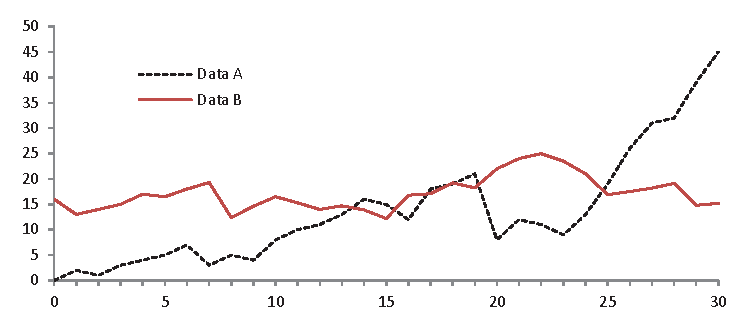
\includegraphics{fig1.eps}" the figure file must be called
\verb"fig1.eps" and not \verb"Fig1.eps" or \verb"fig1.EPS".  If you are on a Unix system, please ensure that
there are no pairs of figures whose names differ only in capitalization, such as \verb"fig_2a.eps" and \verb"fig_2A.eps",
as Windows systems will be unable to keep the two files in the same directory.
\end{itemize}
When you submit your article files, they are manipulated
and copied many times across multiple databases and file systems. Including non-standard
characters in your filenames will cause problems when processing your article.
\subsubsection{\label{fname}Naming your figure files.} In addition to the above points, please give each figure file a name which indicates the number of the figure it contains; for example, \verb"figure1.eps", \verb"figure2a.eps", etc. If the figure file contains a figure with multiple parts, for example figure 2(a) to 2(e), give it a name such as \verb"figure2a_2e.eps", and so forth.
\subsection{How to send your files}
Please send your submission via the ScholarOne submission system.  Go to the journal home
page, and use the `Submit an article' link on the right-hand side.

\section{Preparing your article}

\subsection{Sample coding for the start of an article}
\label{startsample}
The code for the start of a title page of a typical paper in the \verb"iopart.cls" style might read:
\small\begin{verbatim}
\documentclass[12pt]{iopart}
\begin{document}
\title[The anomalous magnetic moment of the 
neutrino]{The anomalous magnetic moment of the 
neutrino and its relation to the solar neutrino problem}

\author{P J Smith$^1$, T M Collins$^2$, 
R J Jones$^3$\footnote{Present address:
Department of Physics, University of Bristol, Tyndalls Park Road, 
Bristol BS8 1TS, UK.} and Janet Williams$^3$}

\address{$^1$ Mathematics Faculty, Open University, 
Milton Keynes MK7~6AA, UK}
\address{$^2$ Department of Mathematics, 
Imperial College, Prince Consort Road, London SW7~2BZ, UK}
\address{$^3$ Department of Computer Science, 
University College London, Gower Street, London WC1E~6BT, UK}
\ead{williams@ucl.ac.uk}

\begin{abstract}
...
\end{abstract}
\keywords{magnetic moment, solar neutrinos, astrophysics}
\submitto{\jpg}
\maketitle
\end{verbatim}
\normalsize

At the start of the \LaTeX\ source code please include 
commented material to identify the journal, author, and (if you are sending a revised
version or a resubmission) the reference number that the journal
has given to the submission. The first non-commented line should be 
\verb"\documentclass[12pt]{iopart}"  to load the preprint class 
file.  The normal text will be in the Computer Modern 12pt font.
It is possible to specify 10pt font size by passing the option \verb"[10pt]" to the class file.
Although it is possible to choose a font other than Computer Modern by loading external packages, this is not recommended.

The article text begins after \verb"\begin{document}".
Authors of very long articles may find it convenient to separate 
their article into a series of \LaTeX\ files each containing one section, and each of which is called 
in turn by the primary file.  The files for each section should be read in from the current directory;
please name the primary file clearly so that we know to run \LaTeX\ on this file.

Authors may use any common \LaTeX\ \verb".sty" files.
Authors may also define their own macros and definitions either in the main article \LaTeX\ file
or in a separate \verb".tex" or \verb".sty" file that is read in by the
main file, provided they do not overwrite existing definitions.
It is helpful to the production staff if complicated author-defined macros are explained in a \LaTeX\ comment.
The article class \verb"iopart.cls" can be used with other package files such
as those loading the AMS extension fonts 
\verb"msam" and \verb"msbm", which provide the 
blackboard bold alphabet and various extra maths symbols as well as symbols useful in figure 
captions.  An extra style file \verb"iopams.sty" is provided to load these
packages and provide extra definitions for bold Greek letters.

\subsection{\label{dblcol}Double-column layout}
The \verb"iopart.cls" class file produces single-column output by default, but a two-column layout can be obtained by
using \verb"\documentclass[10pt]" at the start of the file and \verb"\ioptwocol" after the \verb"\maketitle" command.  Two-column output will begin
on a new page (unlike in published double-column articles, where the two-column material
starts on the same page as the abstract).

In general we prefer to receive submissions in single-column format even for journals
published in double-column style; however, the \verb"\ioptwocol" option may be useful to test figure sizes
and equation breaks for these journals.  When setting material
in two columns you can use the asterisked versions of \LaTeX\ commands such as \verb"\begin{figure*} ... \end{figure*}"
to set figures and tables across two columns.  If you have any problems or any queries about producing two-column output, please contact us at \verb"submissions@iop.org".

\section{The title and abstract page} 
If you use \verb"iopart.cls", the code for setting the title page information is slightly different from
the normal default in \LaTeX.  If you are using a different class file, you do not need to mimic the appearance of
an \verb"iopart.cls" title page, but please ensure that all of the necessary information is present.

\subsection{Titles and article types}
The title is set using the command
\verb"\title{#1}", where \verb"#1" is the title of the article. The
first letter 
of the title should be capitalized with the rest in lower case. 
The title appears in bold case, but mathematical expressions within the title may be left in light-face type. 

If the title is too long to use as a running head at the top of each page (apart from the
first) a short
form can be provided as an optional argument (in square brackets)
before the full title, i.e.\ \verb"\title[Short title]{Full title}".

For article types other than papers, \verb"iopart.cls"
has a generic heading \verb"\article[Short title]{TYPE}{Full title}" 
and some specific definitions given in table~\ref{arttype}. In each case (apart from Letters
to the Editor and Fast Track Communications) an 
optional argument can be used immediately after the control sequence name
to specify the short title; where no short title is given, the full title
will be used as the running head.  Not every article type has its own macro---use \verb"\article" for
any not listed.  A full list of the types of articles published by a journal is given
in the submission information available via the journal home page.
%For Letters use \verb"\letter{Full title}"; no short title is required as 
%the running head is automatically defined to be {\it Letter to the Editor}.
The generic heading could be used for 
articles such as those presented at a conference or workshop, e.g.
\small\begin{verbatim}
\article[Short title]{Workshop on High-Energy Physics}{Title}
\end{verbatim}\normalsize
Footnotes to titles may be given by using \verb"\footnote{Text of footnote.}" immediately after the title.
Acknowledgment of funding should be included in the acknowledgments section rather than in a footnote.

\begin{table}
\caption{\label{arttype}Types of article defined in the {\tt iopart.cls} 
class file.}
\footnotesize\rm
\begin{tabular*}{\textwidth}{@{}l*{15}{@{\extracolsep{0pt plus12pt}}l}}
\br
Command& Article type\\
\mr
\verb"\title{#1}"&Paper (no surtitle on first page)\\
\verb"\ftc{#1}"&Fast Track Communication\\
\verb"\review{#1}"&Review\\
\verb"\topical{#1}"&Topical Review\\
\verb"\comment{#1}"&Comment\\
\verb"\note{#1}"&Note\\
\verb"\paper{#1}"&Paper (no surtitle on first page)\\
\verb"\prelim{#1}"&Preliminary Communication\\
\verb"\rapid{#1}"&Rapid Communication\\
\verb"\letter{#1}"&Letter to the Editor\\
\verb"\article{#1}{#2}"&Other articles\\\ & (use this for any other type of article; surtitle is whatever is entered as {\tt 
\#1})\\
\br
\end{tabular*}
\end{table}

\subsection{Authors' names and addresses}
For the authors' names type \verb"\author{#1}", 
where \verb"#1" is the 
list of all authors' names. Western-style names should be written as initials then
family name, with a comma after all but the last 
two names, which are separated by `and'. Initials should {\it not} be followed by full stops. First (given) names may be used if 
desired.  Names in Chinese, Japanese and Korean styles should be written as you want them to appear in the published article. Authors in all IOP Publishing journals have the option to include their names in Chinese, Japanese or Korean characters in addition to the English name: see appendix B for details. 


If the authors are at different addresses a superscripted number, e.g. $^1$, \verb"$^1$", should be used after each 
name to reference the author to his/her address.
If an author has additional information to appear as a footnote, such as 
a permanent address, a normal \LaTeX\ footnote command
should be given after the family name and address marker 
with this extra information.

The authors' affiliations follow the list of authors. 
Each address is set by using
\verb"\address{#1}" with the address as the single parameter in braces. 
If there is more 
than one address then the appropriate superscripted number, followed by a space, should come at the start of
the address.
 
E-mail addresses are added by inserting the 
command \verb"\ead{#1}" after the postal address(es) where \verb"#1" is the e-mail address.  
See section~\ref{startsample} for sample coding. For more than one e-mail address, please use the command 
\verb"\eads{\mailto{#1}, \mailto{#2}}" with \verb"\mailto" surrounding each e-mail address.  Please ensure
that, at the very least, you state the e-mail address of the corresponding author.

\subsection{The abstract}
The abstract follows the addresses and
should give readers concise information about the content 
of the article and indicate the main results obtained and conclusions 
drawn. It should be self-contained---there should be no references to 
figures, tables, equations, bibliographic references etc.  It should be enclosed between \verb"\begin{abstract}"
and \verb"\end{abstract}" commands.  The abstract should normally be restricted 
to a single paragraph of around 200 words.

\subsection{Subject classification numbers}
We no longer ask authors to supply Physics and Astronomy Classification System (PACS)
classification numbers.  For submissions to {\it Nonlinearity}\/ we ask that you should
supply Mathematics Subject Classification (MSC) codes.  MSC numbers are included after the abstract 
using \verb"\ams{#1}".

The command
\verb"\submitto{#1}" can be inserted, where \verb"#1" is the journal name written in full or the appropriate control sequence as
given in table~\ref{jlab1}. This command is not essential to the running of the file and can be omitted.

\subsection{Keywords}
Keywords are required for all submissions. Authors should supply a minimum of three (maximum seven) keywords appropriate to their article as a new paragraph starting \verb"\noindent{\it Keywords\/}:" after the end of the abstract.

\subsection{Making a separate title page}
To keep the header material on a separate page from the
body of the text insert \verb"\maketitle" (or \verb"\newpage") before the start of the text. 
If \verb"\maketitle" is not included the text of the
article will start immediately after the abstract.  

\section{The text}
\subsection{Sections, subsections and subsubsections}
The text of articles may be divided into sections, subsections and, where necessary, 
subsubsections. To start a new section, end the previous paragraph and 
then include \verb"\section" followed by the section heading within braces. 
Numbering of sections is done {\it automatically} in the headings: 
sections will be numbered 1, 2, 3, etc, subsections will be numbered 
2.1, 2.2,  3.1, etc, and subsubsections will be numbered 2.3.1, 2.3.2, 
etc.  Cross references to other sections in the text should, where
possible, be made using 
labels (see section~\ref{xrefs}) but can also
be made manually. See section~\ref{eqnum} for information on the numbering of displayed equations. Subsections and subsubsections are 
similar to sections but 
the commands are \verb"\subsection" and \verb"\subsubsection" respectively. 
Sections have a bold heading, subsections an italic heading and 
subsubsections an italic heading with the text following on directly.
\small\begin{verbatim}
\section{This is the section title}
\subsection{This is the subsection title}
\end{verbatim}\normalsize

The first section is normally an introduction,  which should state clearly 
the object of the work, its scope and the main advances reported, with 
brief references to relevant results by other workers. In long papers it is 
helpful to indicate the way in which the paper is arranged and the results 
presented.

Footnotes should be avoided whenever possible and can often be included in the text as phrases or sentences in parentheses. If required, they should be used only for brief notes that do not fit conveniently into the text. The use of 
displayed mathematics in footnotes should be avoided wherever possible and no equations within a footnote should be numbered. 
The standard \LaTeX\ macro \verb"\footnote" should be used.  Note that in \verb"iopart.cls" the \verb"\footnote" command
produces footnotes indexed by a variety of different symbols,
whereas in published articles we use numbered footnotes.  This
is not a problem: we will convert symbol-indexed footnotes to numbered ones during the production process.

\subsection{Acknowledgments}
Authors wishing to acknowledge assistance or encouragement from 
colleagues, special work by technical staff or financial support from 
organizations should do so in an unnumbered `Acknowledgments' section 
immediately following the last numbered section of the paper. In \verb"iopart.cls" the 
command \verb"\ack" sets the acknowledgments heading as an unnumbered
section.

Please ensure that you include all of the sources of funding and the funding contract reference numbers that you are contractually obliged to acknowledge. We often receive requests to add such information very late in the production process, or even after the article is published, and we cannot always do this. Please collect all of the necessary information from your co-authors and sponsors as early as possible.  

\subsection{Appendices}
Technical detail that it is necessary to include, but that interrupts 
the flow of the article, may be consigned to an appendix. 
Any appendices should be included at the end of the main text of the paper, after the acknowledgments section (if any) but before the reference list.
If there are 
two or more appendices they should be called Appendix A, Appendix B, etc. 
Numbered equations will be in the form (A.1), (A.2), etc,
figures will appear as figure A1, figure B1, etc and tables as table A1,
table B1, etc.

The command \verb"\appendix" is used to signify the start of the
appendices. Thereafter \verb"\section", \verb"\subsection", etc, will 
give headings appropriate for an appendix. To obtain a simple heading of 
`Appendix' use the code \verb"\section*{Appendix}". If it contains
numbered equations, figures or tables the command \verb"\appendix" should
precede it and \verb"\setcounter{section}{1}" must follow it. 
 
\subsection{Some matters of style}
It will help the readers if your article is written in a clear,
consistent and concise manner. During the production process
we will try to make sure that your work is presented to its
readers in the best possible way without sacrificing the individuality of
your writing. Some recommended 
points to note, however, are the following.  These apply to all of the journals listed
in table~\ref{jlab1}.
\begin{enumerate}
\item Authors are often inconsistent in the use of `ize' and `ise' endings.
We recommend using `-ize' spellings (diagonalize, 
renormalization, minimization, etc) but there are some common 
exceptions to this, for example: devise, 
promise and advise.

\item The words table and figure should be written 
in full and {\bf not} abbreviaged to tab. and fig. Do not include `eq.', `equation' etc before an equation number or `ref.'\, `reference' etc before a reference number.
\end{enumerate}

Please check your article carefully for accuracy, consistency and clarity before
submission. Remember that your article will probably be read by many
people whose native language is not English and who may not  
be aware of many of the subtle meanings of words or idiomatic phases
present in the English language. It therefore helps if you try to keep
sentences as short and simple as possible.  If you are not a native English speaker,
please ask a native English speaker to read your paper and check its grammar.

\section{Mathematics}
\subsection{Two-line constructions}
The great advantage of \LaTeX\ 
over other text processing systems is its 
ability to handle mathematics of almost any degree of complexity. However, 
in order to produce an article suitable for publication both within a print journal and online, 
authors should exercise some restraint on the constructions used. Some equations using very small characters which are clear in a preprint style article may be difficult read in a smaller format.

For simple fractions in the text the solidus \verb"/", as in 
$\lambda/2\pi$, should be used instead of \verb"\frac" or \verb"\over", 
using parentheses where necessary to avoid ambiguity, 
for example to distinguish between $1/(n-1)$ and $1/n-1$. Exceptions to 
this are the proper fractions $\frac12$, $\frac13$, $\frac34$, 
etc, which are better left in this form. In displayed equations 
horizontal lines are preferable to solidi provided the equation is 
kept within a height of two lines. A two-line solidus should be 
avoided where possible; the construction $(\ldots)^{-1}$ should be 
used instead. For example use:
\begin{equation*}
\frac{1}{M_{\rm a}}\left(\int^\infty_0{\rm d}
\omega\;\frac{|S_o|^2}{N}\right)^{-1}\qquad\mbox{instead of}\qquad
\frac{1}{M_{\rm a}}\biggl/\int^\infty_0{\rm d}
\omega\;\frac{|S_o|^2}{N}.
\end{equation*}

\subsection{Roman and italic in mathematics}
In mathematics mode \LaTeX\ automatically sets variables in an italic 
font. In most cases authors should accept this italicization. However, 
there are some cases where it is preferable to use a Roman font; for 
instance, a Roman d for a differential d, a Roman e 
for an exponential e and a Roman i for the square root of $-1$. To 
accommodate this and to simplify the  typing of equations, \verb"iopart.cls" provides
some extra definitions. \verb"\rmd", \verb"\rme" and \verb"\rmi" 
now give Roman d, e and i respectively for use in equations, 
e.g.\ $\rmi x\rme^{2x}\rmd x/\rmd y$ 
is obtained by typing \verb"$\rmi x\rme^{2x}\rmd x/\rmd y$". 
 

Certain other common mathematical functions, such as cos, sin, det and 
ker, should appear in Roman type. Standard \LaTeX\ provides macros for 
most of these functions 
(in the cases above, \verb"\cos", \verb"\sin", \verb"\det" and \verb"\ker" 
respectively); \verb"iopart.cls" also provides 
additional definitions for $\Tr$, $\tr$ and 
$\Or$ (\verb"\Tr", \verb"\tr" and \verb"\Or", respectively). 

Subscripts and superscripts should be in Roman type if they are labels 
rather than variables or characters that take values. For example in the 
equation
\[
\epsilon_m=-g\mu_{\rm n}Bm
\]
$m$, the $z$ component of the nuclear spin, is italic because it can have 
different values whereas n is Roman because it 
is a label meaning nuclear ($\mu_{\rm n}$ 
is the nuclear magneton).


\subsection{Displayed equations in double-column journals}
Authors should bear in mind that all mathematical formulae in double-column journals will need to fit
into the width of a single column.  You may find it helpful to use a two-column layout (such as the two-column
option in \verb"iopart.cls") in your submission so that you can check the width of equations.

\subsection{Special characters for mathematics}
Bold italic characters can be used in our journals to signify vectors (rather
than using an upright bold or an over arrow). To obtain this effect when using \verb"iopart.cls",
use \verb"\bi{#1}" within maths mode, e.g. $\bi{ABCdef}$. Similarly, in \verb"iopart.cls", if upright 
bold characters are required in maths, use \verb"\mathbf{#1}" within maths
mode, e.g. $\mathbf{XYZabc}$. The calligraphic (script) uppercase alphabet
is obtained with \verb"\mathcal{AB}" or \verb"\cal{CD}" 
($\mathcal{AB}\cal{CD}$).

The American Mathematical Society provides a series of extra symbol fonts
to use with \LaTeX\ and packages containing the character definitions to
use these fonts. Authors wishing to use Fraktur 
\ifiopams$\mathfrak{ABC}$ \fi
or Blackboard Bold \ifiopams$\mathbb{XYZ}$ \fi can include the appropriate
AMS package (e.g. \verb"amsgen.sty", \verb"amsfonts.sty", \verb"amsbsy.sty", \verb"amssymb.sty") with a 
\verb"\usepackage" command or add the command \verb"\usepackage{iopams}"
which loads the four AMS packages mentioned above and also provides
definitions for extra bold characters (all Greek letters and some other
additional symbols). 

The package \verb"iopams.sty" uses the definition \verb"\boldsymbol" in \verb"amsbsy.sty"
which allows individual non-alphabetical symbols and Greek letters to be 
made bold within equations.
The bold Greek lowercase letters \ifiopams$\balpha \ldots\bomega$,\fi 
are obtained with the commands 
\verb"\balpha" \dots\ \verb"\bomega" (but note that
bold eta\ifiopams, $\bfeta$,\fi\ is \verb"\bfeta" rather than \verb"\beta")
and the capitals\ifiopams, $\bGamma\ldots\bOmega$,\fi\ with commands 
\verb"\bGamma" \dots\
\verb"\bOmega". Bold versions of the following symbols are
predefined in \verb"iopams.sty": 
bold partial\ifiopams, $\bpartial$,\fi\ \verb"\bpartial",
bold `ell'\ifiopams, $\bell$,\fi\  \verb"\bell", 
bold imath\ifiopams, $\bimath$,\fi\  \verb"\bimath", 
bold jmath\ifiopams, $\bjmath$,\fi\  \verb"\bjmath", 
bold infinity\ifiopams, $\binfty$,\fi\ \verb"\binfty", 
bold nabla\ifiopams, $\bnabla$,\fi\ \verb"\bnabla", 
bold centred dot\ifiopams, $\bdot$,\fi\  \verb"\bdot". Other 
characters are made bold using 
\verb"\boldsymbol{\symbolname}".

Please do not use the style file \verb"amsmath.sty" (part of the AMSTeX package) in conjunction with \verb"iopart.cls". This will result in several errors. To make use of the macros defined in \verb"amsmath.sty", \verb"iopart.cls" provides the file \verb"setstack.sty" which reproduces the following useful macros from \verb"amsmath.sty":
\small\begin{verbatim}
\overset \underset \sideset \substack \boxed   \leftroot
\uproot  \dddot    \ddddot  \varrow   \harrow
\end{verbatim}\normalsize

If the mathematical notation
that you need is best handled in \verb"amsmath.sty" you might want to consider using an article class
other than \verb"iopart.cls". We accept submissions using any class or style files.

Table~\ref{math-tab2} lists some other macros for use in 
mathematics with a brief description of their purpose.

\begin{table}
\caption{\label{math-tab2}Other macros defined in {\tt iopart.cls} for use in maths.}
\begin{tabular*}{\textwidth}{@{}l*{15}{@{\extracolsep{0pt plus
12pt}}l}}
\br
Macro&Result&Description\\
\mr
\verb"\fl"&&Start line of equation full left\\
\verb"\case{#1}{#2}"&$\case{\#1}{\#2}$&Text style fraction in display\\
\verb"\Tr"&$\Tr$&Roman Tr (Trace)\\
\verb"\tr"&$\tr$&Roman tr (trace)\\
\verb"\Or"&$\Or$&Roman O (of order of)\\
\verb"\tdot{#1}"&$\tdot{x}$&Triple dot over character\\
\verb"\lshad"&$\lshad$&Text size left shadow bracket\\
\verb"\rshad"&$\rshad$&Text size right shadow bracket\\
\br
\end{tabular*}
\end{table}

\subsection{Alignment of displayed equations}

The normal style for aligning displayed equations in our published journal articles is to align them left rather than centre. The \verb"iopart.cls" class file automatically does this and indents each line of a display.  In \verb"iopart.cls", to make any line start at the left margin of the page, add \verb"\fl" at start of the line (to indicate full left).

Using the \verb"eqnarray" environment equations will naturally be aligned left and indented without the use of any ampersands for alignment, see equations (\ref{eq1}) and (\ref{eq2})
\begin{eqnarray}
\alpha + \beta =\gamma^2, \label{eq1}\\
\alpha^2 + 2\gamma + \cos\theta = \delta. \label{eq2} 
\end{eqnarray}
This is the normal equation style for our journals.

Where some secondary alignment is needed, for instance a second part of an equation on a second line, a single ampersand is added at the point of alignment in each line  (see  (\ref{eq3}) and (\ref{eq4})).
\begin{eqnarray}
\alpha &=2\gamma^2 + \cos\theta + \frac{XY \sin\theta}{X+ Y\cos\theta} \label{eq3}\\
 & = \delta\theta PQ \cos\gamma. \label{eq4} 
\end{eqnarray}
 
Two points of alignment are possible using two ampersands for alignment (see  (\ref{eq5}) and (\ref{eq6})).  Note in this case extra space \verb"\qquad" is added before the second ampersand in the longest line (the top one) to separate the condition from the equation. 
\begin{eqnarray}
\alpha &=2\gamma^2 + \cos\theta + \frac{XY \sin\theta}{X+ Y\cos\theta}\qquad& \theta > 1 \label{eq5}\\
 & = \delta\theta PQ \cos\gamma &\theta \leq 1.\label{eq6} 
\end{eqnarray}

For a long equation which has to be split over more than one line the first line should start at the left margin, this is achieved by inserting \verb"\fl" (full left) at the start of the line. The use of the alignment parameter \verb"&" is not necessary unless some secondary alignment is needed.
\begin{eqnarray}
\fl \alpha + 2\gamma^2 = \cos\theta + \frac{XY \sin\theta}{X+ Y\cos\theta} +  \frac{XY \sin\theta}{X- Y\cos\theta} +
+ \left(\frac{XY \sin\theta}{X+ Y\cos\theta}\right)^2 \nonumber\\
+  \left(\frac{XY \sin\theta}{X- Y\cos\theta}\right)^2.\label{eq7} 
\end{eqnarray}

The plain \TeX\ command \verb"\eqalign" can be used within an \verb"equation" environment to obtain a multiline equation with a single centred number, for example
\begin{equation}
\eqalign{\alpha + \beta =\gamma^2 \cr
\alpha^2 + 2\gamma + \cos\theta = \delta.} 
\end{equation}

During the production process we will break equations as appropriate for the page layout of the journal. If you are submitting to a double-column journal and wish to review how your equations will break, you may find the double-column layout described in section \ref{dblcol} useful.
 
\subsection{Miscellaneous points}
The following points on the layout of mathematics apply whichever class file you use.

Exponential expressions, especially those containing subscripts or 
superscripts, are clearer if the notation $\exp(\ldots)$ is used, except for 
simple examples. For instance $\exp[\rmi(kx-\omega t)]$ and $\exp(z^2)$ are 
preferred to $\e^{\rmi(kx-\omega t)}$ and $\e^{z^2}$, but 
$\e^x$ 
is acceptable. 

Similarly the square root sign $\sqrt{\phantom{b}}$ should 
only be used with relatively
simple expressions, e.g.\ $\sqrt2$ and $\sqrt{a^2+b^2}$;
in other cases the 
power $1/2$ should be used; for example, $[(x^2+y^2)/xy(x-y)]^{1/2}$.

It is important to distinguish between $\ln = \log_\e$ and $\lg 
=\log_{10}$. Braces, brackets and parentheses should be used in the 
following order: $\{[(\;)]\}$. The same ordering of brackets should be 
used within each size. However, this ordering can be ignored if the
brackets have a 
special meaning (e.g.\ if they denote an average or a function).  

Decimal fractions should always be preceded by a zero: for example 0.123 {\bf not} .123.
For long numbers use thin spaces after every third character away from the position of the decimal point, unless 
this leaves a single separated character: e.g.\ $60\,000$, $0.123\,456\,78$ 
but 4321 and 0.7325.

Equations should be followed by a full stop (periods) when at the end
of a sentence.

\subsection{Equation numbering and layout in {\tt iopart.cls}}
\label{eqnum}
\LaTeX\ provides facilities for automatically numbering equations 
and these should be used where possible. Sequential numbering (1), (2), 
etc, is the default numbering system although in \verb"iopart.cls", if the command
\verb"\eqnobysec" is included in the preamble, equation numbering
by section is obtained, e.g.\ 
(2.1), (2.2), etc. Equation numbering by section is used in appendices automatically when the \verb"\appendix" command is used, even if sequential numbering has been used in the rest of the article. 
Refer to equations in the text using the equation number in parentheses. It is not normally necessary to include the word equation before the number; and abbreviations such as eqn or eq should not be used.
In \verb"iopart.cls", there are alternatives to the standard \verb"\ref" command that you might
find useful---see \tref{abrefs}.

Sometimes it is useful to number equations as parts of the same
basic equation. This can be accomplished in \verb"iopart.cls" by inserting the 
commands \verb"\numparts" before the equations concerned and 
\verb"\endnumparts" when reverting to the normal sequential numbering.
For example using \verb"\numparts \begin{eqnarray}" ... \verb"\end{eqnarray} \endnumparts":

\numparts
\begin{eqnarray}
T_{11}&=(1+P_\e)I_{\uparrow\uparrow}-(1-P_\e)
I_{\uparrow\downarrow},\label{second}\\
T_{-1-1}&=(1+P_\e)I_{\downarrow\downarrow}-(1-P_\e)I_{\uparrow\downarrow},\\
S_{11}&=(3+P_\e)I_{\downarrow\uparrow}-(3-P_e)I_{\uparrow\uparrow},\\
S_{-1-1}&=(3+P_\e)I_{\uparrow\downarrow}-(3-P_\e)
I_{\downarrow\downarrow}.
\end{eqnarray}
\endnumparts

Equation labels within the \verb"\eqnarray" environment will be referenced
as subequations, e.g. (\ref{second}).

\subsection{Miscellaneous extra commands for displayed equations}
The \verb"\cases" command has been amended slightly in \verb"iopart.cls" to 
increase the space between the equation and the condition. 
\Eref{cases} 
demonstrates simply the output from the \verb"\cases" command
\begin{equation}
\label{cases}
X=\cases{1&for $x \ge 0$\\
-1&for $x<0$\\}
\end{equation}
%The code used was:
%\small\begin{verbatim}
%\begin{equation}
%\label{cases}
%X=\cases{1&for $x \ge 0$\\
%-1&for $x<0$\\}
%\end{equation}
%\end{verbatim}
%\normalsize

To obtain text style fractions within displayed maths the command 
\verb"\case{#1}{#2}" can be used instead
of the usual \verb"\frac{#1}{#2}" command or \verb"{#1 \over #2}".

When two or more short equations are on the same line they should be 
separated by a `qquad space' (\verb"\qquad"), rather than
\verb"\quad" or any combination of \verb"\,", \verb"\>", \verb"\;" 
and \verb"\ ".

\section{Referencing\label{except}}
Two different styles of referencing are in common use: 
the Harvard alphabetical system and the Vancouver numerical system. 
All journals to which this document applies allow the use of either the Harvard or Vancouver system, 
except for {\it Physics in Medicine and Biology} and {\it Physiological Measurement}
for which authors {\it must\/} use the Harvard referencing style (with the titles of journal
articles given, and final page numbers given). 

\subsection{Harvard (alphabetical) system}
In the Harvard system the name of the author appears in the text together 
with the year of publication. As appropriate, either the date or the name 
and date are included within parentheses. Where there are only two authors 
both names should be given in the text; if there are more than two 
authors only the first name should appear followed by `{\it et al}' 
(which can be obtained in \verb"iopart.cls" by typing \verb"\etal"). When two or 
more references to work by one author or group of authors occur for the 
same year they should be identified by including a, b, etc after the date 
(e.g.\ 2012a). If several references to different pages of the same article 
occur the appropriate page number may be given in the text, e.g.\ Kitchen 
(2011, p 39).

The reference list at the end of an article consists of an 
unnumbered `References' section containing an
alphabetical listing by authors' names. References with the same author list are ordered by date, oldest first.
The reference list in the 
preprint style is started in \verb"iopart.cls" by including the command \verb"\section*{References}" and then
\verb"\begin{harvard}".
Individual references start with \verb"\item[]" and the reference list is completed with \verb"\end{harvard}".
There is also a shortened form of the coding: \verb"\section*{References}"
and \verb"\begin{harvard}" can be replaced by the single command
\verb"\References", and \verb"\end{harvard}" can be shortened to
\verb"\endrefs".

\subsection{Vancouver (numerical) system}
In the Vancouver system references are numbered sequentially 
throughout the text. The numbers occur within square brackets and one 
number can be used to designate several references. A numerical 
reference list in the \verb"iopart" style is started by including the 
command \verb"\section*{References}" and then
\verb"\begin{thebibliography}{<num>}", where \verb"<num>" is the largest
number in the reference list (or any other number with the same number
of digits).  The 
reference list gives the references in 
numerical order, individual references start with \verb"\bibitem{label}". The list is completed by
\verb"\end{thebibliography}". Short forms of the commands are again
available: \verb"\Bibliography{<num>}" can be used at the start of the
references section and \verb"\endbib" at the end.

A variant of this system is to use labels instead of numbers within 
square brackets, in this case references in the list should start with \verb"\bibitem[label-text]". This method is allowed for all journals that accept numerical references.

\subsection{BibTeX\label{bibtex}}
If you are using BibTeX, see the earlier section \ref{bibby} for information on what \verb".bst" file to use.
The output that you get will differ slightly from that specified in the rest of this section,
but this is not a problem as long as all the relevant information is present.

\subsection{References, general}
A complete reference should provide the reader with enough information to 
locate the item concerned. Up to ten authors may be given in a particular reference; where 
there are more than ten only the first should be given followed by 
`{\it et al}'.  If you are using BibTeX
and the \verb".bst" file that you are using includes more than 10 authors, do not worry about this:
we can correct this during the production process.  Abbreviate a journal name only in accordance with the journal's
own recommendations for abbreviation---if in doubt, leave it unabbreviated.

The terms {\it loc.\ cit.}\ and {\it ibid}.\ should not be used. 
Unpublished conferences and reports should generally not be included 
in the reference list if a published version of the work exists. Articles in the course of publication should 
include the article title and the journal of publication, if known. 
A reference to a thesis submitted for a higher degree may be included 
if it has not been superseded by a published 
paper---please state the institution where the work was submitted.

The basic structure of a reference in the reference list is the same in both the alphabetical and numerical systems, the only difference being the code at the start of the reference. Alphabetical references are preceded by \verb"\item[]", numerical by \verb"\bibitem{label}" or just \verb"\item" to generate a number or \verb"\nonum" where a reference is not the first in a group of references under the same number.

Note that footnotes to the text should not be 
included in the reference list, but should appear at the bottom of the relevant page by using the \verb"\footnote" command.
   
\subsection{References to journal articles}
The following guidance applies if you are producing your reference list `by hand'; that is,
without the help of BibTeX.  See section~\ref{bibby} for BibTeX help.

Article references in published articles in our journals contain three changes of 
font:
the authors and date appear in Roman type, the journal title in 
italic, the volume number in bold and the page numbers in Roman again. 
A typical journal entry would be:

\smallskip
\begin{harvard}
\item[] Spicer P E, Nijhoff F W and van der Kamp P H 2011 {\it Nonlinearity} {\bf 24} 2229
\end{harvard}
\smallskip

\noindent which would be obtained by typing, within the references
environment 
\small\begin{verbatim}
\item[] Spicer P E, Nijhoff F W and van der Kamp P H 2011 {\it Nonlinearity} 
{\bf 24} 2229
\end{verbatim}\normalsize

\noindent Features to note are the following.

\begin{enumerate}
\item The authors should be in the form of surname (with only the first 
letter capitalized) followed by the initials with no 
periods after the initials. Authors should be separated by a comma 
except for the last two which should be separated by `and' with no 
comma preceding it.

\item The year of publication follows the authors and is not in parentheses.  

\item Titles of journal articles can also be included (in Roman (upright) text after the year). Article titles are required in reference lists for {\it Inverse Problems, Journal of Neural Engineering, Measurement Science and Technology, Physical Biology, Physics in Medicine and Biology\/} and {\it Physiological Measurement}.

\item The journal is in italic and is abbreviated. If a journal has several parts denoted by 
different letters the part letter should be inserted after the journal in Roman type (e.g.\ 
{\it Phys.\ Rev.\ \rm A}). \verb"iopart.cls" includes macros for abbreviated titles of all journals handled by IOP Publishing (see table~\ref{jlab2}) and some other common titles (table \ref{jlab3}). 

\item The volume number is bold; the page number is Roman.
 Both the initial and final page numbers should be given where possible---note that for {\it Reports on Progress in Physics\/}, {\it Physiological Measurement} and {\it Physics in Medicine and Biology}
 the final page number is {\it required}. The final page number should be in 
the shortest possible form and separated from the initial page number by an en rule (\verb"--"), e.g.\ 1203--14.

\item Where there are two or more references with identical authors, 
the authors' names should be repeated for the second and subsequent references. Each individual publication should be presented as a separate reference, although in the numerical system one number can be used for several references. This facilitates linking in the online journal. 
\end{enumerate}


\subsubsection{Article numbering.}
Many journals now use article-numbering systems that do not fit the conventional {\it year-journal-volume-page numbers} pattern. Some examples are:

\numrefs{1}
\item Carlip S and Vera R 1998 {\it Phys. Rev.} D {\bf 58} 011345 
\item Davies K and Brown G 1997 {\it J. High Energy Phys.} JHEP12(1997)002
\item Hannestad S 2005 {\it J. Cosmol. Astropart. Phys.} JCAP02(2005)011
\item Hilhorst H J 2005 {\it J. Stat. Mech.} L02003
\item Gundlach C 1999 {\it Liv. Rev. Rel.} 1994-4
\endnumrefs

\noindent The website of the journal you are citing should state the correct format for citations.

\subsection{Preprint references}
Preprints may be referenced but if the article concerned has been published in a peer-reviewed journal, that reference should take precedence. If only a preprint reference can be given, it is helpful to include the article title. Examples are:
\vskip6pt
\numrefs{1}
\item Neilson D and Choptuik M 2000 {\it Class. Quantum Grav.} {\bf 17} 761 (arXiv:gr-qc/9812053)
\item Sundu H, Azizi K, S\"ung\"u J Y and Yinelek N 2013 Properties of $D_{s2}^*(2573)$ charmed-strange tensor meson arXiv:1307.6058
\endnumrefs

\noindent For preprints added to arXiv.org after April 2007 it is not necessary to include the subject area, however this information can be included in square brackets after the number if desired, e.g.
\numrefs{1}
\item Sundu H, Azizi K, S\"ung\"u J Y and Yinelek N 2013 Properties of $D_{s2}^*(2573)$ charmed-strange tensor meson arXiv:1307.6058 [hep-ph]
\endnumrefs

\subsection{References to books, conference proceedings and reports}

References to books, proceedings and reports are similar, but have only two
changes of font. The authors and date of publication are in Roman, the 
title of the book is in italic, and the editors, publisher, 
town of publication 
and page number are in Roman. A typical reference to a book and a
conference paper might be

\smallskip
\begin{harvard}
\item[] Dorman L I 1975 {\it Variations of Galactic Cosmic Rays} 
(Moscow: Moscow State University Press) p~103
\item[] Caplar R and Kulisic P 1973 {\it Proc.\
Int.\ Conf.\ on Nuclear Physics (Munich)} vol~1 (Amsterdam:  
North-Holland/American Elsevier) p~517
\end{harvard}
\smallskip

\noindent which would be obtained by with the code
\small\begin{verbatim}
\item[] Dorman L I 1975 {\it Variations of Galactic Cosmic Rays} 
(Moscow: Moscow State University Press) p~103
\item[] Caplar R and Kulisic P 1973 {\it Proc. Int. Conf. on Nuclear 
Physics (Munich)} vol~1 (Amsterdam: North-Holland/American 
Elsevier) p~517
\end{verbatim}\normalsize
\noindent 

\noindent Features to note are the following.
\begin{enumerate}
\item Book titles are in italic and should be spelt out in full with 
initial capital letters for all except minor words. Words such as 
Proceedings, Symposium, International, Conference, Second, etc should 
be abbreviated to Proc., Symp., Int., Conf., 2nd, 
respectively, but the rest of the title should be given in full, 
followed by the date of the conference and the 
town or city where the conference was held. For 
laboratory reports the laboratory should be spelt out wherever 
possible, e.g.\ {\it Argonne National Laboratory Report}.

\item The volume number, for example, vol~2, should be followed by 
the editors, if any, in the form ed~A~J~Smith and P~R~Jones. Use 
\etal if there are more than two editors. Next comes the town of 
publication and publisher, within brackets and separated by a colon, 
and finally the page numbers preceded by p if only one number is given 
or pp if both the initial and final numbers are given.

\item If a book is part of a series (for examples, {\it Springer Tracts in Modern Physics\/}), the series title and volume number is given in parentheses after the book title. Whereas for an individual volume in a multivolume set, the set title is given first, then the volume title. 
\end{enumerate}
\smallskip
\begin{harvard}
\item[]Morse M 1996 Supersonic beam sources {\it Atomic Molecular and Optical Physics\/} ({\it Experimental Methods in the Physical Sciences\/} vol 29) ed F B Dunning and R Hulet (San Diego, CA: Academic)  
\item[]Fulco C E, Liverman C T and Sox H C (eds) 2000 {\it Gulf War and Health\/} vol 1 {\it Depleted Uranium, Pyridostigmine Bromide, Sarin, and Vaccines\/} (Washington, DC: The National Academies Press)
\end{harvard}

\section{Cross-referencing\label{xrefs}}
The facility to cross reference items in the text is very useful when 
composing articles as the precise form of the article may be uncertain at the start 
and  revisions and amendments may subsequently be made. 
\LaTeX\ provides excellent facilities for doing cross-referencing
and these can be very useful in preparing articles.

\subsection{References}
\label{refs}
Cross referencing is useful for numeric reference lists because, if it 
is used, adding 
another reference to the list does not then involve renumbering all 
subsequent references. It is not necessary for referencing 
in the Harvard system where the final reference list is alphabetical 
and normally no other changes are necessary when a reference is added or
deleted.
When using \LaTeX , two passes (under certain circumstances, three passes)
are necessary initially to get the cross references right 
but once they are correct a single run is usually sufficient provided an 
\verb".aux" file is available and the file 
is run to the end each time.
If the 
reference list contains an entry \verb"\bibitem{label}", 
this command 
will produce the correct number in the reference list and 
\verb"\cite{label}" will produce the number within square brackets in the 
text. \verb"label" may contain letters, numbers 
or punctuation characters but must not contain spaces or commas. It is also
recommended that the underscore character \_{} is not used in cross
referencing. 
Thus labels of the form 
\verb"eq:partial", \verb"fig:run1", \verb"eq:dy'", 
etc, may be used. When several 
references occur together in the text \verb"\cite" may be used with 
multiple labels with commas but no spaces separating them; 
the output will be the 
numbers within a single pair of square brackets with a comma and a 
thin space separating the numbers. Thus \verb"\cite{label1,label2,label4}"
would give [1,\,2,\,4]. Note that no attempt is made by the style file to sort the 
labels and no shortening of groups of consecutive numbers is done.
Authors should therefore either try to use multiple labels in the correct 
order, or use a package such as \verb"cite.sty" that reorders labels
correctly.

The numbers for the cross referencing are generated in the order the 
references appear in the reference list, so that if the entries in the 
list are not in the order in which the references appear in the text 
then the 
numbering within the text will not be sequential. To correct this 
change the ordering of the entries in the reference list and then 
rerun the \LaTeX\ file {\it twice}.  Please ensure that all references resolve correctly: check the \verb".log" file
for undefined or multiply-defined citations, and check that the output does not contain question
marks that indicate unresolved references.

\subsection{Equation numbers, sections, subsections, figures and 
tables}
Labels for equation numbers, sections, subsections, figures and tables 
are all defined with the \verb"\label{label}" command and cross references 
to them are made with the \verb"\ref{label}" command. 

Any section, subsection, subsubsection, appendix or subappendix 
command defines a section type label, e.g. 1, 2.2, A2, A1.2 depending 
on context. A typical article might have in the code of its introduction 
`The results are discussed in section\verb"~\ref{disc}".' and
the heading for the discussion section would be:
\small\begin{verbatim}
\section{Results}\label{disc}
\end{verbatim}\normalsize
Labels to sections, etc, may occur anywhere within that section except
within another numbered environment. 
Within a maths environment labels can be used to tag equations which are 
referred to within the text. 

In addition to the standard \verb"\ref{<label>}", in \verb"iopart.cls" the abbreviated
forms given in \tref{abrefs}
are available for reference to standard parts of the text.

\Table{\label{abrefs}Alternatives to the normal references command {\tt $\backslash$ref} available in {\tt iopart.cls},
and the text generated by
them. Note it is not normally necessary to include the word equation
before an equation number except where the number starts a sentence. The
versions producing an initial capital should only be used at the start of
sentences.} 
\br
Reference&Text produced\\
\mr
\verb"\eref{<label>}"&(\verb"<num>")\\
\verb"\Eref{<label>}"&Equation (\verb"<num>")\\
\verb"\fref{<label>}"&figure \verb"<num>"\\
\verb"\Fref{<label>}"&Figure \verb"<num>"\\
\verb"\sref{<label>}"&section \verb"<num>"\\
\verb"\Sref{<label>}"&Section \verb"<num>"\\
\verb"\tref{<label>}"&table \verb"<num>"\\
\verb"\Tref{<label>}"&Table \verb"<num>"\\
\br
\endTable

\section{Tables and table captions}
Tables are numbered serially and referred to in the text 
by number (table 1, etc, {\bf not} tab. 1). Each table should have an 
explanatory caption which should be as concise as possible. If a table 
is divided into parts these should be labelled \pt(a), \pt(b), 
\pt(c), etc but there should be only one caption for the whole 
table, not separate ones for each part.

In the preprint style the tables may be included in the text 
or listed separately after the reference list 
starting on a new page. 

\subsection{The basic table format}
The standard form for a table in \verb"iopart.cls" is:
\small\begin{verbatim}
\begin{table}
\caption{\label{label}Table caption.}
\begin{indented}
\item[]\begin{tabular}{@{}llll}
\br
Head 1&Head 2&Head 3&Head 4\\
\mr
1.1&1.2&1.3&1.4\\
2.1&2.2&2.3&2.4\\
\br
\end{tabular}
\end{indented}
\end{table}
\end{verbatim}\normalsize

\noindent Points to note are:
\begin{enumerate}
\item The caption comes before the table. It should have a period at
the end.

\item Tables are normally set in a smaller type than the text.
The normal style is for tables to be indented. This is accomplished
by using \verb"\begin{indented}" \dots\ \verb"\end{indented}"
and putting \verb"\item[]" before the start of the tabular environment.
Omit these
commands for any tables which will not fit on the page when indented.

\item The default is for columns to be aligned left and 
adding \verb"@{}" omits the extra space before the first column.

\item Tables have only horizontal rules and no vertical ones. The rules at
the top and bottom are thicker than internal rules and are set with
\verb"\br" (bold rule). 
The rule separating the headings from the entries is set with
\verb"\mr" (medium rule).  These are special \verb"iopart.cls" commands.

\item Numbers in columns should be aligned on the decimal point;
to help do this a control sequence \verb"\lineup" has been defined
in \verb"iopart.cls"
which sets \verb"\0" equal to a space the size of a digit, \verb"\m"
to be a space the width of a minus sign, and \verb"\-" to be a left
overlapping minus sign. \verb"\-" is for use in text mode while the other
two commands may be used in maths or text.
(\verb"\lineup" should only be used within a table
environment after the caption so that \verb"\-" has its normal meaning
elsewhere.) See table~\ref{tabone} for an example of a table where
\verb"\lineup" has been used.
\end{enumerate}

\begin{table}
\caption{\label{tabone}A simple example produced using the standard table commands 
and $\backslash${\tt lineup} to assist in aligning columns on the 
decimal point. The width of the 
table and rules is set automatically by the 
preamble.} 

\begin{indented}
\lineup
\item[]\begin{tabular}{@{}*{7}{l}}
\br                              
$\0\0A$&$B$&$C$&\m$D$&\m$E$&$F$&$\0G$\cr 
\mr
\0\023.5&60  &0.53&$-20.2$&$-0.22$ &\01.7&\014.5\cr
\0\039.7&\-60&0.74&$-51.9$&$-0.208$&47.2 &146\cr 
\0123.7 &\00 &0.75&$-57.2$&\m---   &---  &---\cr 
3241.56 &60  &0.60&$-48.1$&$-0.29$ &41   &\015\cr 
\br
\end{tabular}
\end{indented}
\end{table}

\subsection{Simplified coding and extra features for tables}
The basic coding format can be simplified using extra commands provided in
the \verb"iopart" class file. The commands up to and including 
the start of the tabular environment
can be replaced by
\small\begin{verbatim}
\Table{\label{label}Table caption}
\end{verbatim}\normalsize
and this also activates the definitions within \verb"\lineup".
The final three lines can also be reduced to \verb"\endTable" or
\verb"\endtab". Similarly for a table which does not fit on the page when indented
\verb"\fulltable{\label{label}caption}" \dots\ \verb"\endfulltable"
can be used. \LaTeX\ optional positional parameters can, if desired, be added after 
\verb"\Table{\label{label}caption}" and \verb"\fulltable{\label{label}caption}".


\verb"\centre{#1}{#2}" can be used to centre a heading 
\verb"#2" over \verb"#1" 
columns and \verb"\crule{#1}" puts a rule across 
\verb"#1" columns. A negative 
space \verb"\ns" is usually useful to reduce the space between a centred 
heading and a centred rule. \verb"\ns" should occur immediately after the 
\verb"\\" of the row containing the centred heading (see code for
\tref{tabl3}). A small space can be 
inserted between rows of the table 
with \verb"\ms" and a half line space with \verb"\bs" 
(both must follow a \verb"\\" but should not have a 
\verb"\\" following them).
   
\Table{\label{tabl3}A table with headings spanning two columns and containing notes. 
To improve the 
visual effect a negative skip ($\backslash${\tt ns})
has been put in between the lines of the 
headings. Commands set-up by $\backslash${\tt lineup} are used to aid 
alignment in columns. $\backslash${\tt lineup} is defined within
the $\backslash${\tt Table} definition.}
\br
&&&\centre{2}{Separation energies}\\
\ns
&Thickness&&\crule{2}\\
Nucleus&(mg\,cm$^{-2}$)&Composition&$\gamma$, n (MeV)&$\gamma$, 2n (MeV)\\
\mr
$^{181}$Ta&$19.3\0\pm 0.1^{\rm a}$&Natural&7.6&14.2\\
$^{208}$Pb&$\03.8\0\pm 0.8^{\rm b}$&99\%\ enriched&7.4&14.1\\
$^{209}$Bi&$\02.86\pm 0.01^{\rm b}$&Natural&7.5&14.4\\
\br
\end{tabular}
\item[] $^{\rm a}$ Self-supporting.
\item[] $^{\rm b}$ Deposited over Al backing.
\end{indented}
\end{table}

Units should not normally be given within the body of a table but 
given in brackets following the column heading; however, they can be 
included in the caption for long column headings or complicated units. 
Where possible tables should not be broken over pages. 
If a table has related notes these should appear directly below the table
rather than at the bottom of the page. Notes can be designated with
footnote symbols (preferable when there are only a few notes) or
superscripted small roman letters. The notes are set to the same width as
the table and in normal tables follow after \verb"\end{tabular}", each
note preceded by \verb"\item[]". For a full width table \verb"\noindent"
should precede the note rather than \verb"\item[]". To simplify the coding 
\verb"\tabnotes" can, if desired, replace \verb"\end{tabular}" and 
\verb"\endtabnotes" replaces
\verb"\end{indented}\end{table}".

If all the tables are grouped at the end of a document
the command \verb"\Tables" is used to start a new page and 
set a heading `Tables and table captions'. If the tables follow an appendix then add the command \verb"\noappendix" to revert to normal style numbering.
  
\section{Figures and figure captions}

Figures (with their captions) can be incorporated into the text at the appropriate position or grouped together
at the end of the article. If the figures are at the end of the article and follow an appendix then in \verb"iopart.cls" you can add the command \verb"\noappendix" to revert to normal style numbering.  We remind you that you must seek permission
to reuse any previously-published figures, and acknowledge their use correctly---see section \ref{copyright}.

\subsection{Inclusion of graphics files\label{figinc}}
Using the \verb"graphicx" package graphics files can 
be included within figure and center environments at an 
appropriate point within the text using code such as:
\small\begin{verbatim}
\includegraphics{file.eps}
\end{verbatim}\normalsize
The \verb"graphicx" package supports various optional arguments
to control the appearance of the figure. Other similar 
packages can also be used (e.g. \verb"graphics", \verb"epsf").   Whatever package you use,
you must include it explicitly after the \verb"\documentclass" declaration using (say)
\verb"\usepackage{graphicx}".

For more detail about graphics inclusion see the documentation 
of the \verb"graphicx" package, refer to one of the books on \LaTeX , e.g. Goosens M, Rahtz S and Mittelbach F 1997 {\it The }\LaTeX\ {\it Graphics Companion\/} 
(Reading, MA: Addison-Wesley),
or download some of the excellent free documentation available via the Comprehensive
TeX Archive Network (CTAN) \verb"http://www.ctan.org"---{in particular see Reckdahl K 2006 {\it Using Imported Graphics in }\LaTeX\ {\it and }pdf\LaTeX\ \verb"http://www.ctan.org/tex-archive/info/epslatex".

IOP Publishing's graphics guidelines provide further information on preparing \verb".eps" files.

We prefer you to use \verb".eps" files for your graphics, but we realise that converting other
formats of graphics to \verb".eps" format can be troublesome.  If you use PDF or bitmap-format graphics
such as JPG or PNG that need to be included using the pdf\TeX\ package, this is OK, but please bear
in mind that the PDF you submit should use PDF standard 1.4 or lower (use \verb"\pdfminorversion=4" at the
start of the file).

The main \LaTeX\ file must read in graphics files and subsidiary \LaTeX\ files from the current directory,
{\it not} from a subdirectory.  Your submission files are stored on our systems in a single location and we will not be able to process your
TeX file automatically if it relies on organization of the files into subdirectories.

\subsection{Captions}
Below each figure should be a brief caption describing it and, if 
necessary, interpreting the various lines and symbols on the figure. 
As much lettering as possible should be removed from the figure itself 
and included in the caption. If a figure has parts, these should be 
labelled ($a$), ($b$), ($c$), etc and all parts should be described 
within a single caption. \Tref{blobs} gives the definitions for describing 
symbols and lines often used within figure captions (more symbols are 
available when using the optional packages loading the AMS extension fonts).

\subsection{Supplementary Data}
All of our journals encourage authors to submit supplementary data attachments to 
enhance the online versions of published research articles. Supplementary data 
enhancements typically consist of video clips, animations or
data files, tables of extra information or extra figures. They can 
add to the reader's understanding and present results in attractive ways that go 
beyond what can be presented in the PDF version of the article. 
See our supplementary data guidelines for further details.

Software, in the form of input scripts for mathematical packages (such as Mathematica notebook files), or
source code that can be interpreted or compiled (such as Python scripts or Fortran or C programs), or executable
files, can sometimes be accepted as supplementary data, but the journal may ask you for assurances about
the software and distribute them from the article web page only subject to a disclaimer.  Contact the journal
in the first instance if you want to submit software.

\begin{table}[t]
\caption{\label{blobs}Control sequences to describe lines and symbols in figure 
captions.}
\begin{indented}
\item[]\begin{tabular}{@{}lllll}
\br
Control sequence&Output&&Control sequence&Output\\
\mr
\verb"\dotted"&\dotted        &&\verb"\opencircle"&\opencircle\\
\verb"\dashed"&\dashed        &&\verb"\opentriangle"&\opentriangle\\
\verb"\broken"&\broken&&\verb"\opentriangledown"&\opentriangledown\\
\verb"\longbroken"&\longbroken&&\verb"\fullsquare"&\fullsquare\\
\verb"\chain"&\chain          &&\verb"\opensquare"&\opensquare\\
\verb"\dashddot"&\dashddot    &&\verb"\fullcircle"&\fullcircle\\
\verb"\full"&\full            &&\verb"\opendiamond"&\opendiamond\\
\br
\end{tabular}
\end{indented}
\end{table}

\clearpage

\appendix


\section{List of macros for formatting text, figures and tables}

\begin{table}[hb]
\caption{Macros available for use in text in {\tt iopart.cls}. Parameters in square brackets are optional.}
\footnotesize\rm
\begin{tabular}{@{}*{7}{l}}
\br
Macro name&Purpose\\
\mr
\verb"\title[#1]{#2}"&Title of article and short title (optional)\\
\verb"\paper[#1]{#2}"&Title of paper and short title (optional)\\
\verb"\letter{#1}"&Title of Letter to the Editor\\
\verb"\ftc{#1}"&Title of Fast Track Communication\\
\verb"\rapid[#1]{#2}"&Title of Rapid Communication and short title (optional)\\
\verb"\comment[#1]{#2}"&Title of Comment and short title (optional)\\
\verb"\topical[#1]{#2}"&Title of Topical Review and short title 
(optional)\\
\verb"\review[#1]{#2}"&Title of review article and short title (optional)\\
\verb"\note[#1]{#2}"&Title of Note and short title (optional)\\
\verb"\prelim[#1]{#2}"&Title of Preliminary Communication \& short title\\
\verb"\author{#1}"&List of all authors\\
\verb"\article[#1]{#2}{#3}"&Type and title of other articles and 
short title (optional)\\
\verb"\address{#1}"&Address of author\\
\verb"\ams{#1}"&Mathematics Classification Scheme\\
\verb"\submitto{#1}"&`Submitted to' message\\
\verb"\maketitle"&Creates title page\\
\verb"\begin{abstract}"&Start of abstract\\
\verb"\end{abstract}"&End of abstract\\
\verb"\nosections"&Inserts space before text when no sections\\
\verb"\section{#1}"&Section heading\\
\verb"\subsection{#1}"&Subsection heading\\
\verb"\subsubsection{#1}"&Subsubsection heading\\
\verb"\appendix"&Start of appendixes\\
\verb"\ack"&Acknowledgments heading\\
\verb"\References"&Heading for reference list\\
\verb"\begin{harvard}"&Start of alphabetic reference list\\
\verb"\end{harvard}"&End of alphabetic reference list\\
\verb"\begin{thebibliography}{#1}"&Start of numeric reference list\\
\verb"\end{thebibliography}"&End of numeric reference list\\
\verb"\etal"&\etal for text and reference lists\\
\verb"\nonum"&Unnumbered entry in numerical reference list\\
\br
\end{tabular}
\end{table}

\clearpage

\begin{table}
\caption{Macros defined within {\tt iopart.cls}
for use with figures and tables.}
\begin{indented}
\item[]\begin{tabular}{@{}l*{15}{l}}
\br
Macro name&Purpose\\
\mr
\verb"\Figures"&Heading for list of figure captions\\
\verb"\Figure{#1}"&Figure caption\\
\verb"\Tables"&Heading for tables and table captions\\
\verb"\Table{#1}"&Table caption\\
\verb"\fulltable{#1}"&Table caption for full width table\\
\verb"\endTable"&End of table created with \verb"\Table"\\
\verb"\endfulltab"&End of table created with \verb"\fulltable"\\
\verb"\endtab"&End of table\\
\verb"\br"&Bold rule for tables\\
\verb"\mr"&Medium rule for tables\\
\verb"\ns"&Small negative space for use in table\\
\verb"\centre{#1}{#2}"&Centre heading over columns\\
\verb"\crule{#1}"&Centre rule over columns\\
\verb"\lineup"&Set macros for alignment in columns\\
\verb"\m"&Space equal to width of minus sign\\
\verb"\-"&Left overhanging minus sign\\
\verb"\0"&Space equal to width of a digit\\
\br
\end{tabular}
\end{indented}
\end{table}

\clearpage

\begin{table}[hb]
\caption{\label{jlab2}Abbreviations in {\tt iopart.cls} for journals handled by IOP Publishing.}
\footnotesize
\begin{tabular}{@{}llll}
\br
{\rm Short form of journal title} & Macro & {\rm Short form of journal title} & Macro \\
\mr
2D Mater.&\verb"\TDM"&J. Radiol. Prot.&\verb"\JRP"\\
AJ&\verb"\AJ"&J. Semicond.&\verb"\JOS"\\
ApJ&\verb"\APJ"&J. Stat. Mech.&\verb"\JSTAT"\\
ApJL&\verb"\APJL"&Laser Phys.&\verb"\LP"\\
ApJS&\verb"\APJS"&Laser Phys. Lett.&\verb"\LPL"\\
Adv. Nat. Sci: Nanosci. Nanotechnol.&\verb"\ANSN"&Metrologia&\verb"\MET"\\
Appl. Phys. Express&\verb"\APEX"&Mater. Res. Express&\verb"\MRE"\\
Biofabrication&\verb"\BF"&Meas. Sci. Technol.&\verb"\MST"\\
Bioinspir. Biomim.&\verb"\BB"&Methods Appl. Fluoresc.&\verb"\MAF"\\
Biomed. Mater.&\verb"\BMM"&Modelling Simul. Mater. Sci. Eng.&\verb"\MSMSE"\\
Chin. J. Chem. Phys.&\verb"\CJCP"&Nucl. Fusion&\verb"\NF"\\
Chinese Phys. B&\verb"\CPB"&New J. Phys.&\verb"\NJP"\\
Chinese Phys. C&\verb"\CPC"&Nonlinearity&\verb"\NL"\\
Chinese Phys. Lett.&\verb"\CPL"&Nanotechnology&\verb"\NT"\\
Class. Quantum Grav.&\verb"\CQG"&Phys. Biol.&\verb"\PB"\\
Commun. Theor. Phys.&\verb"\CTP"&Phys. Educ.&\verb"\PED"\\
Comput. Sci. Disc.&\verb"\CSD"&Phys.-Usp.&\verb"\PHU"\\
Environ. Res. Lett.&\verb"\ERL"&Physiol. Meas.&\verb"\PM"\\
EPL&\verb"\EPL"&Phys. Med. Biol.&\verb"\PMB"\\
Eur. J. Phys.&\verb"\EJP"&Phys. Scr.&\verb"\PS"\\
Fluid Dyn. Res.&\verb"\FDR"&Plasma Phys. Control. Fusion&\verb"\PPCF"\\
Inverse Problems&\verb"\IP"&Plasma Sci. Technol.&\verb"\PST"\\
Izv. Math.&\verb"\IZV"&Plasma Sources Sci. Technol.&\verb"\PSST"\\
Jpn. J. Appl. Phys.&\verb"\JJAP"&Quantum Electron.&\verb"\QEL"\\
J. Breath Res.&\verb"\JBR"&Rep. Prog. Phys.&\verb"\RPP"\\
JCAP&\verb"\JCAP"&Res. Astron. Astrophys.&\verb"\RAA"\\
J. Geophys. Eng.&\verb"\JGE"&Russ. Chem. Rev.&\verb"\RCR"\\
JINST&\verb"\JINST"&Russ. Math. Surv.&\verb"\RMS"\\
J. Micromech. Microeng.&\verb"\JMM"&Sb. Math.&\verb"\MSB"\\
J. Neural Eng.&\verb"\JNE"&Science Foundation in China&\verb"\SFC"\\
J. Opt.&\verb"\JOPT"&Sci. Technol. Adv. Mater.&\verb"\STAM"\\
J. Phys. A: Math. Theor.&\verb"\jpa"&Semicond. Sci. Technol.&\verb"\SST"\\
J. Phys. B: At. Mol. Opt. Phys.&\verb"\jpb"&Smart Mater. Struct.&\verb"\SMS"\\
J. Phys: Condens. Matter&\verb"\JPCM"&Supercond. Sci. Technol.&\verb"\SUST"\\
J. Phys. D: Appl. Phys.&\verb"\JPD"&Surf. Topogr.: Metrol. Prop.&\verb"\STMP"\\
J. Phys. G: Nucl. Part. Phys.&\verb"\jpg"&Transl. Mater. Res.&\verb"\TMR"\\
\mr
{\it IOP Conference Series journals}\\
\mr
J. Phys.: Conf. Ser.&\verb"\JPCS"\\
IOP Conf. Ser.: Earth Environ. Sci.&\verb"\EES"\\
IOP Conf. Ser.: Mater. Sci. Eng.&\verb"\MSE"\\

\br
\end{tabular}

\end{table}

\clearpage

\begin{table}

\caption{\label{jlab2b}Abbreviations for IOP Publishing journals that are no longer published.}
\begin{indented}
\item[]\begin{tabular}{@{}lll}
\br
{\rm Short form of journal title} & Macro name & Years relevant\\
\mr
J. Phys. A: Math. Gen.&\verb"\JPA"&1975--2006\\
J. Phys. B: At. Mol. Phys.&\verb"\JPB"&1968--1987\\
J. Phys. C: Solid State Phys.&\verb"\JPC"&1968--1988\\
J. Phys. E: Sci. Instrum.&\verb"\JPE"&1968--1989\\
J. Phys. F: Met. Phys.&\verb"\JPF"&1971--1988\\
J. Phys. G: Nucl. Phys.&\verb"\JPG"&1975--1988\\
Pure Appl. Opt.&\verb"\PAO"&1992--1998\\
Quantum Opt.&\verb"\QO"&1989--1994\\
Quantum Semiclass. Opt.&\verb"\QSO"&1995--1998\\
J. Opt. A: Pure Appl. Opt.&\verb"\JOA"&1999--2009\\
J. Opt. B: Quantum Semiclass. Opt.&\verb"\JOB"&1999--2005\\
\br
\end{tabular}
\end{indented}
\end{table}

\begin{table}[h]

\caption{\label{jlab3}Abbreviations in {\tt iopart.cls} for some 
common journals not handled by IOP Publishing.}
\begin{indented}
\item[]\begin{tabular}{@{}llll}
\br
Short form of journal & Macro & Short form of Journal & Macro\\
\mr
Acta Crystallogr.&\verb"\AC"&J. Quant. Spectrosc. Radiat. Transfer&\verb"\JQSRT"\\
Acta Metall.&\verb"\AM"&Nuovo Cimento&\verb"\NC"\\
Ann. Phys., Lpz&\verb"\AP"&Nucl. Instrum. Methods&\verb"\NIM"\\
Ann. Phys., NY&\verb"\APNY"&Nucl. Phys.&\verb"\NP"\\
Ann. Phys., Paris&\verb"\APP"&Phys. Fluids&\verb"\PF"\\
Can. J. Phys.&\verb"\CJP"&Phys. Lett.&\verb"\PL"\\
Gen. Rel. Grav.&\verb"\GRG"&Phys. Rev.&\verb"\PR"\\
J. Appl. Phys.&\verb"\JAP"&Phys. Rev. Lett.&\verb"\PRL"\\
J. Chem. Phys.&\verb"\JCP"&Proc. R. Soc.&\verb"\PRS"\\
J. High Energy Phys.&\verb"\JHEP"&Phys. Status Solidi&\verb"\PSS"\\
J. Magn. Magn. Mater.&\verb"\JMMM"&Phil. Trans. R. Soc.&\verb"\PTRS"\\
J. Math. Phys.&\verb"\JMP"&Rev. Mod. Phys.&\verb"\RMP"\\
J. Opt. Soc. Am.&\verb"\JOSA"&Rev. Sci. Instrum.&\verb"\RSI"\\
J. Physique&\verb"\JP"&Solid State Commun.&\verb"\SSC"\\
J. Phys. Chem.&\verb"\JPhCh"&Sov. Phys.--JETP&\verb"\SPJ"\\
J. Phys. Soc. Jpn.&\verb"\JPSJ"&Z. Phys.&\verb"\ZP"\\


\br
\end{tabular}
\end{indented}
\end{table}

\clearpage

\section{Including author names using Chinese, Japanese and Korean characters in submissions to IOP Publishing journals}
Authors in all IOP Publishing journals have the option to include names in Chinese, Japanese or Korean (CJK) characters in addition to the English name. The names will be displayed in the print issue and the online PDF, abstract and table of contents, in parentheses after the English name. 

It is the decision of the individual authors whether or not to include a CJK version of their names; for a single article it is not necessary for all authors to include a CJK name if only one author wishes to do so. It is the responsibility of the authors to check the accuracy and formatting of the names in the final proofs that they receive prior to publication. 

To include names in CJK characters, authors should use the \verb"cjk.sty" package, available from \verb"http://www.ctan.org/tex-archive/language/chinese/CJK/". Users should be aware that this is a very large and complicated package which relies on a large number of fonts.  We recommend using a TeX package that includes this package and all of the fonts by default, so that manual configuration is not required (e.g. the TeXLive distribution, which is available on all platforms (Macintosh, Windows and Linux)).

The documentation for the \verb"cjk.sty" package gives information on how CJK characters can be included in TeX files.  Most authors will find it convenient to include the characters in one of the standard encodings such as UTF-8, GB or JIS, if they have access to a text editor that supports such encodings.

Example TeX coding might be:
\begin{verbatim}
\documentclass[12pt]{iopart}
\usepackage{CJK}
.
.
.
\begin{document}
\begin{CJK*}{GBK}{ }

\title[]{Title of article}
\author{Author Name (CJK characters)}
\address{Department, University, City, Country}
.
.
.
\end{CJK*}
\end{verbatim}

To avoid potential problems in handling the CJK characters in submissions, authors should always include a PDF of the full version of their papers (including all figure files, tables, references etc) with the CJK characters in it.


\end{document}

